\chapter{Funcionamento e tecnologias}
\label{chap:funcionamento}

\enlargethispage{-.5\baselineskip}

\section{Processo de desenvolvimento}
   Durante o período de desenvolvimento, a equipe adotou a Metodologia Ágil. Dada a complexidade do processo de desenvolvimento de software, a utilização de um modelo único mostrou-se insuficiente e ineficaz. A abordagem ágil foi escolhida devido aos benefícios de sua natureza adaptativa e personalizada, proporcionando não apenas desenvolvimento mais rápido e eficaz, mas também maturidade à organização, conforme discutido por \cite{8229928}.

    Nesse contexto, os principais marcos temporais do ciclo de desenvolvimento foram estabelecidos como Milestones. Em resumo, esses marcos representam metas específicas a serem alcançadas em momentos determinados, auxiliando na divisão do processo em fases gerenciáveis. Isso permite o acompanhamento do progresso e a avaliação do cumprimento de objetivos em momentos-chave.

   \begin{figure}[!htb]
       \centering
       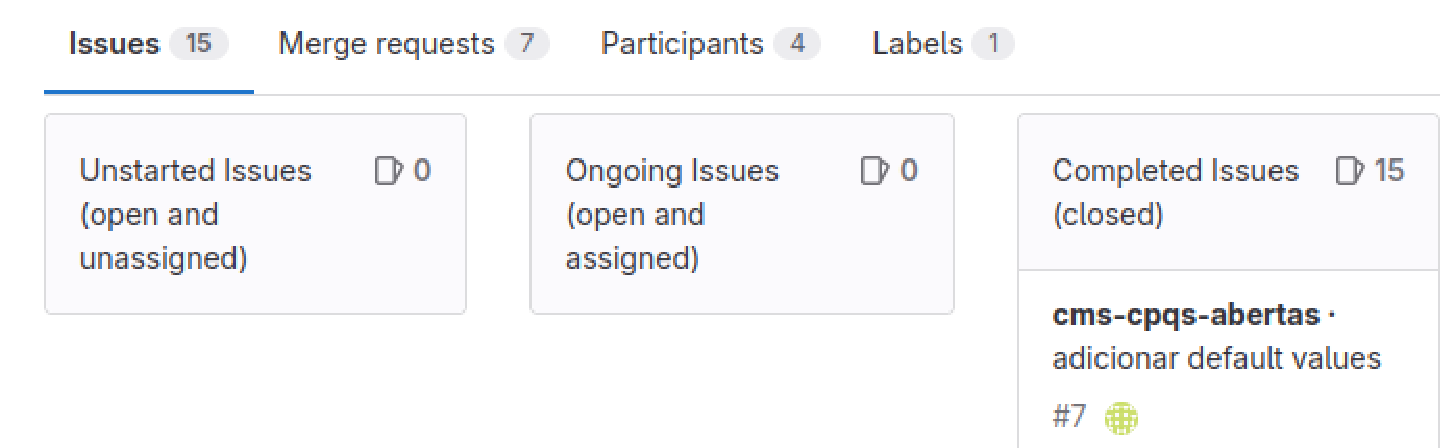
\includegraphics[width=0.75\textwidth]{figuras/milestones.pdf}
       \caption{Milestone: visualização Scrum Board}
       \label{milestones}
    \end{figure}

 Além disso, dentro de cada Milestone, a administração era conduzida por meio da visualização em forma de Scrum Board, conforme ilustrado em \ref{milestones}. Essa ferramenta visual geralmente consiste em colunas representando etapas como "To Do", "In Progress" e "Done". Dessa forma, foi possível obter uma visão rápida do status de cada issue ou tarefa.

As issues ou tarefas, por sua vez, podem se referir a bugs, melhorias ou qualquer unidade de trabalho identificada e registrada no sistema de controle e gerenciamento. É importante ressaltar que não havia um formato padrão de issue: algumas eram abrangentes e continham subitens para auxiliar no entendimento, enquanto outras eram curtas e gerais.

Para cada issue realizada, o código referente à melhoria era adicionado a uma branch, ou seja, a uma versão independente do código-fonte no repositório do Gitlab. Esse uso permitiu que todos os desenvolvedores da equipe trabalhassem em recursos separados sem interferir uns nos outros.

Ao concluir a issue, era efetuado um Pull Request, ou seja, uma solicitação para incorporar as alterações de uma branch ao código principal. A aprovação dessas requisições ocorria após a realização do code review, prática essencial em metodologias ágeis. Esse método envolve a revisão sistemática e colaborativa do código por outros membros da equipe. Durante cada revisão, o membro responsável garantia que o código estivesse em conformidade com os padrões de codificação, diretrizes e práticas estabelecidas pela equipe.

\section{Strapi}
Como mencionado em seções anteriores, a estratégia adotada para avançar no desenvolvimento do projeto foi a utilização do Headless CMS, com destaque para a abordagem empregada pelo Strapi. O Strapi é uma ferramenta de gerenciamento de conteúdo de código aberto que utiliza Node.js. Seu papel central inclui a disponibilização de APIs e a organização dos conteúdos de maneira clara e intuitiva.

Na atual paisagem de desenvolvimento web, a gestão de conteúdo digital desempenha um papel fundamental na construção de sites e aplicativos interativos e dinâmicos. O Strapi destaca-se como uma solução notável e inovadora nesse cenário, oferecendo um sistema de gerenciamento de conteúdo de código aberto que se diferencia por sua flexibilidade, personalização e capacidade de criar e gerenciar APIs robustas. Projetado para atender às necessidades dos desenvolvedores modernos que buscam uma abordagem mais flexível na gestão de conteúdo, o Strapi permite que os desenvolvedores criem, modifiquem e organizem facilmente o conteúdo digital conforme as especificações de seus projetos. Essa flexibilidade é alcançada por meio de uma arquitetura de plugin extensível, que facilita a adição de funcionalidades personalizadas de maneira simples e eficaz.

Uma das características mais distintivas do Strapi é sua habilidade de gerar automaticamente APIs RESTful e GraphQL com base no conteúdo definido no sistema. Isso implica não apenas a capacidade de criar conteúdo, mas também de expô-lo facilmente para uso em aplicativos web, móveis e outros sistemas. A capacidade de oferecer acesso a dados estruturados por meio de APIs é especialmente valiosa em um mundo digital altamente interconectado. O Strapi foi concebido com interoperabilidade em mente, suportando vários tipos de bancos de dados. Essa abertura possibilita aos desenvolvedores escolher o sistema de armazenamento de dados que melhor se alinha às necessidades de seus projetos, desde bancos de dados SQL tradicionais até soluções NoSQL. Essa flexibilidade é essencial para integrar o Strapi em diversos contextos de desenvolvimento.

Outra vantagem significativa da ferramenta é sua interface de usuário intuitiva e amigável. Isso simplifica a criação e gestão de conteúdo, tornando o Strapi acessível mesmo a usuários não técnicos. No entanto, a plataforma também oferece uma estrutura orientada para desenvolvedores que possibilita personalizações avançadas. Isso garante que as equipes de desenvolvimento possam criar experiências de usuário refinadas e complexas, ao mesmo tempo em que os editores de conteúdo consigam gerenciar o conteúdo de forma fácil, sem depender constantemente de intervenção técnica.

O núcleo do Headless CMS, presente no gerenciador de conteúdo da ferramenta, é onde reside a essência do Strapi. Nele, são listados os chamados 'Collection Types', cuja definição depende do contexto específico do projeto. No caso do CpqsAbertas, por exemplo, temos Institutos e Departamentos como coleções distintas. Nesse contexto, Departamentos representam unidades específicas, como MAT, DCC, MAE, etc., enquanto Institutos servem como representação das faculdades em si, como IME, FAU, FEARP. Cada 'Collection Type' possui campos variados, como texto, JSON, números, relações, entre outros. O preenchimento desses campos é crucial, pois é por meio deles que a API é alimentada.

%%%%%%%%%%%%%%%%%%%%%%%%%%%%%%%%%%%%
%(talvez inserir aqui um print da página do strapi que lista os campos disponíveis para uso)

%%%%%%%%%%%%%%%%%%%%%%%%%%%%5
O Strapi ganhou popularidade em diversos cenários de desenvolvimento web e de aplicativos, sendo frequentemente escolhido para projetos que demandam um alto grau de controle sobre o conteúdo e sua exposição por meio de APIs. Essa escolha abrange uma ampla gama de casos de uso, desde sites corporativos e blogs até aplicativos móveis, lojas online e sistemas de gerenciamento de conteúdo complexos. Essa versatilidade demonstra a adaptabilidade e a eficácia do Strapi em atender às necessidades de diferentes tipos de projetos.

Ao adotar o modelo de arquitetura Headless CMS, por meio da implementação eficaz do Strapi, o Projeto Cpqs-abertas experimentou uma transformação significativa em sua infraestrutura e metodologia de desenvolvimento. A transição de uma abordagem monolítica para uma estrutura mais flexível e desacoplada proporcionou não apenas uma gestão mais eficiente do conteúdo, mas também uma maior adaptabilidade às demandas em constante evolução do projeto. A estratégia "white label" e o uso estratégico de um Sistema de Gerenciamento de Conteúdo (CMS) desempenharam papéis fundamentais na unificação e manutenção contínua do projeto, permitindo que ele cumprisse sua missão de disseminar conhecimento de forma eficaz e colaborativa. A escolha do Strapi, com sua capacidade de gerar APIs automaticamente e oferecer flexibilidade na gestão de conteúdo, destacou-se como um elemento central para alcançar o equilíbrio entre personalização avançada e simplicidade na administração do sistema. Essa seção revela não apenas uma evolução tecnológica, mas também um alinhamento estratégico crucial para o Cpqs-abertas, marcando um capítulo significativo em sua trajetória de desenvolvimento.

\section{Manutenção AWS}

\section{Disseminação Software Livre}
Uma das motivações intrínsecas do projeto, desde a sua concepção, está vinculada à sua participação ativa na comunidade de Software Livre. Seguindo a definição da Free Software Foundation, uma embaixadora desse movimento, o Software Livre proporciona o controle sobre a tecnologia utilizada em nossas residências, escolas e negócios. Este controle visa o benefício individual e coletivo, não sendo submetido a empresas de software proprietário ou governos que buscam restringir e monitorar os usuários.
    
    \begin{quote}
     \enquote{Free software is about having control over the technology we use in our homes, schools and businesses, where computers work for our individual and communal benefit, not for proprietary software companies or governments who might seek to restrict and monitor us.}
    \end{quote}

Nesse contexto, a base essencial para o sucesso de um software na comunidade de Software Livre é sua hospedagem em plataformas de código aberto. Atualmente, as opções mais populares incluem o GitHub, GitLab e Bitbucket. Durante a fundação do projeto CPQs Abertas, esse critério teve influência decisiva na escolha, e o projeto está hospedado no GitLab. Além disso, a escolha da licença é de extrema importância, levando à escolha da MIT, cujas principais características incluem permissividade, reutilização livre e liberdade de uso. Essa licença também é compatível com outras, permitindo sua combinação no mesmo software, inclusive com software proprietário. É vital, no entanto, manter a nota de direitos autorais e a isenção de responsabilidade em todas as cópias do software.

Durante o desenvolvimento, é crucial manter uma documentação abrangente e fornecer um canal de comunicação aberto. No caso do CPQs Abertas, após cada período de trabalho dos grupos, a documentação era obrigatoriamente atualizada para incluir explicações detalhadas sobre instalação, configuração e uso do software. Isso facilitaria a contribuição de novos desenvolvedores para o projeto. No que diz respeito ao canal de comunicação, as issues relacionadas a determinado período eram atualizadas conforme sua execução. Adicionalmente, foi organizado um procedimento para adicionar e documentar cada uma das issues pendentes ao final do período de desenvolvimento, visando facilitar para os próximos desenvolvedores.

Apesar da base existente, o projeto ainda não alcançou o reconhecimento necessário na comunidade de Software Livre, limitando-se ao desenvolvimento por grupos anuais de alunos. Isso destaca a importância de construir uma comunidade mais ampla e promover a disseminação do projeto. Dado o desejo dos fundadores de transformar o projeto em um verdadeiro software de código aberto com contribuições ativas, é imperativo trabalhar nesse aspecto. Para os futuros desenvolvedores da CPQs Abertas, especialmente se não houver a necessidade imediata de lidar com mudanças estruturais, é desejável dedicar esforços nesse sentido. Isso pode ser realizado por meio de palestras, apresentações, participação em conferências relacionadas ao código aberto e divulgação online.

Nesta etapa, para conquistar espaço e visibilidade em mídias de grande alcance, é essencial contar com o apoio de influentes dentro da Universidade, além de obter reconhecimento de todas as unidades da USP. O principal desafio estava relacionado à dificuldade de criar e manter atualizadas novas plataformas web. Administrar várias plataformas simultaneamente sem recursos adequados é inviável. Os recursos implementados pela equipe solucionam questões emergenciais relacionadas à escalabilidade, possibilitando a construção quase imediata de plataformas web para cada unidade. A única barreira é a obtenção dos dados do Lattes, uma vez que a equipe da CPqs Abertas não tem acesso direto a essas informações.

A estratégia de implementação baseada em White Label tem como principal objetivo reduzir os custos de produção, permitindo um foco maior no marketing e divulgação. Com as melhorias implementadas, é razoável afirmar que, a médio prazo, haverá um reconhecimento suficiente por parte da comunidade acadêmica e universitária. Isso abrirá caminho para buscar apoio em mídias de divulgação mais amplas.

Em síntese, a orientação do projeto CPQs Abertas em direção à filosofia do Software Livre, embasada nos princípios de controle tecnológico descentralizado e benefício coletivo, reflete-se na escolha estratégica de plataformas de código aberto, como o GitLab, e na adoção da licença MIT. Estes fundamentos não apenas alinham o projeto com os valores essenciais do movimento, mas também estabelecem uma base sólida para o engajamento e contribuições da comunidade. No entanto, o desafio persiste na ampliação do reconhecimento e participação, sendo essencial explorar estratégias de divulgação em eventos, palestras e meios online. A busca pelo apoio de detentores de poder na Universidade, bem como o aprimoramento constante da infraestrutura técnica, são passos fundamentais para superar as barreiras que limitam o crescimento do projeto. Ao promover uma cultura de Software Livre e fortalecer a comunidade ao seu redor, o CPQs Abertas pode solidificar sua posição como uma contribuição valiosa para a disseminação do conhecimento acadêmico em um contexto aberto e colaborativo.